% IEEE standard conference template; to be used with:
%   spconf.sty  - LaTeX style file, and
%   IEEEbib.bst - IEEE bibliography style file.
% --------------------------------------------------------------------------

\documentclass[letterpaper]{article}
\usepackage{spconf,amsmath,amssymb,graphicx}
\usepackage{xcolor}

\usepackage{hyperref}
\usepackage{fontawesome}
\usepackage{subcaption}
\usepackage{balance}
\usepackage{lipsum}
\usepackage{enumitem}

\newcommand\exthref[2]{\href{#1}{\faicon{share-square-o}~#2}}


% Example definitions.
% --------------------
% nice symbols for real and complex numbers
\newcommand{\R}[0]{\mathbb{R}}
\newcommand{\C}[0]{\mathbb{C}}

% bold paragraph titles
\newcommand{\mypar}[1]{{\bf #1.}}

\newcommand{\TODO}[1]{{\large\textbf{\textcolor{red}{}}}}
\newcommand{\INFO}[1]{{\textbf{\textcolor{orange}{}}}}
% \newcommand{\INFO}[1]{{\textbf{\textcolor{orange}{}}}}
% Title.
% ------
\title{2D/3D Lattice Boltzmann Method Optimization On AMD Zen3}
%
% Single address.
% ---------------
\name{Dominic Wüst, Kamelia Ivanova, Albert Cerfeda, Karlo Piškor}
\address{Department of Computer Science\\ ETH Zurich, Switzerland}

% For example:
% ------------
%\address{School\\
%		 Department\\
%		 Address}
%
% Two addresses (uncomment and modify for two-address case).
% ----------------------------------------------------------
%\twoauthors
%  {A. Author-one, B. Author-two\sthanks{Thanks to XYZ agency for funding.}}
%		 {School A-B\\
%		 Department A-B\\
%		 Address A-B}
%  {C. Author-three, D. Author-four\sthanks{The fourth author performed the work
%		 while at ...}}
%		 {School C-D\\
%		 Department C-D\\
%		 Address C-D}
%

\begin{document}
%\ninept
%
\maketitle
%

% \begin{itemize} 
% 	\item The hard page limit is 7 pages in this style. This excludes references and excludes the short, mandatory part on individual contributions (see end). 
% 	\item No appendix. 
% 	\item Do not reduce font size or use other tricks to squeeze. 
% 	\item The pdf is formatted in the American letter format, so may look a bit strange when printed out (and there is no real reason to do this).
% \end{itemize}

\begin{abstract}

In this project, we explore the Lattice Boltzmann Method which is used for fluid simulations, but can also be applied in various other fields. While the algorithm is already remarkably fast compared to other implementations of fluid simulations, we explore possibilities for further improving performances through better utilization of available resources. The optimizations aren't based on a new model or by tweaking the algorithm's accuracy or output, but rather purely relying on the basis of better resource utilization.



\end{abstract}


\section{Introduction}\label{sec:intro}

% Do not start the introduction with the abstract or a slightly modified
% version. What follows is a possible structure of the introduction.
% This structure can be modified, but the content should be the same. The introduction should definitely end on the first page and leave some space for the second section on the first page.

\mypar{Motivation} 
Simulations are known to be very resource-intensive workloads, making optimizing them essential. This is particularly important for use cases where rapid iterations over multiple scenarios in a model or where one is constrained by available compute resources. In fluid dynamics, precise and effective simulations are crucial for diverse applications, ranging from aerodynamics and weather prediction to biomedical technology and industrial processes. 

Traditional computational fluid dynamics solutions, such as the Navier-Stokes~\cite{navier1838navier} equations, are computationally demanding and can be challenging to implement for complex geometry and boundary conditions~\cite{thibault2009cuda}. This often results in excessively long processing times, making it challenging to do fast prototyping. 

The Lattice Boltzmann Method~\cite{kruger2017lattice} (LBM) offers the advantage of simplified calculations, being easily parallelizable and easily supporting complex collision geometries~\cite{bao2011lattice}. However, despite its advantages, LBM simulations are still computationally expensive, especially for large-scale problems or when high resolution and accuracy are required~\cite{aidun2010lattice}. Therefore, optimizing the performance of LBM simulations is vital for making it more accessible and practical in more applications. An approach shown by N. Delbosc et al.~\cite{DELBOSC2014462} focuses on creating an optimized implementation of the Lattice Boltzmann Method (LBM) with the objective of achieving both real-time computing and satisfactory physical accuracy by leveraging the parallel computation power of GPUs with CUDA. The article mainly discusses the implementation on GPUs and highlights the main obstacles they face throughout their research, mainly boiling down to the high amount of memory accesses in the streaming and collision processes, as well as the GPU-specific issue of significant branch divergence while implementing boundary conditions. 

To ensure the correctness of our implementation we chose a baseline implementation for comparing our results to. For this, we used the 2D LBM implementation from Philip Mocz, available on GitHub~\footnote{2D baseline: \exthref{https://github.com/pmocz/latticeboltzmann-python}{github.com/pmocz/latticeboltzmann-python}}, and the 3D implementation from Callum Marshal, also available on GitHub~\footnote{3D baseline: \exthref{https://github.com/callummarshall9/LBM}{github.com/callummarshall9/LBM}}


% \INFO{The first task is to motivate what you do.  You can
% start general and zoom in one the specific problem you consider.  In
% the process you should have explained to the reader: what you are doing,
% why you are doing, why it is important (order is usually reversed).
% For example, if my result is the fastest DFT implementation ever, one
% could roughly go as follows. First explain why the DFT is important
% (used everywhere with a few examples) and why performance matters (large datasets,
% realtime). Then explain that fast implementations are very hard and
% expensive to get (memory hierarchy, vector, parallel). 
% List some related work on fast implementations for your project if available (in particular those that you compare against) and very briefly explain what they did.}


\mypar{Contribution}
In this paper,  we show that the performance of a trivial implementation of the Lattice Boltzmann Method (LBM) can be significantly enhanced through a series of methodical optimizations applied to standard base implementations. Our project delves into several optimization techniques, including strategies such as code motion, macro expansion, loop blending, precomputation, the use of compiler flags, loop unrolling, shadow indexing, optimizing memory addresses, and vectorization. Specifically for the optimization involving vectorization, we decided to constrain the input size to be divisible by 4. This choice facilitates effective vectorization,  allowing the algorithm full leverage of the CPU's SIMD capabilities. Each of these optimizations was meticulously implemented and tested to ensure they collectively lead to performance gains without compromising the accuracy of the LBM simulations. 


\section{Background on the Algorithm/Application}\label{sec:background}


The Lattice Boltzmann Method (LBM) models fluid flow by modelling the microscopic interactions of particles within a discrete lattice grid. The fundamental components of the LBM algorithm are as follows: 
\begin{enumerate} 
\item \textbf{Streaming Step}: Particles travel to neighbouring lattice sites according to their velocity vectors. This step effectively transfers particle distribution functions across the grid. 
\item \textbf{Collision Step}: At each lattice site, the particle distribution functions undergo a local collision process, redistributing velocities among particles.  This step ensures the preservation of mass and momentum and drives the system toward equilibrium. 
\item \textbf{Boundary Conditions}:  Proper implementation of boundary conditions is essential for accurate simulations. These conditions handle interactions at the domain boundaries, such as walls or in- and outlets, ensuring realistic physical behaviour. In our project we used the periodic boundary condition, according to which an element at the end of the boundary would appear at the opposite side. 
\item \textbf{Distribution Function}: The distribution function represents the ideal state towards which the system evolves during collisions.  It is derived from macroscopic quantities such as density and velocity. 
\item \textbf{Macroscopic Variables Calculation}: The macroscopic fluid properties, such as density and velocity, are computed from the particle distribution function at each lattice site. These quantities are necessary for analyzing the overall fluid behaviour. 
\end{enumerate} 
LBM offers various advantages,  including simplicity, ease of implementation, and inherent parallelism, making it well-suited for high-performance computing environments. Various LBM models exist, such as  D2Q9 and  D3Q15, where "D" indicates the spatial dimension (2D or 3D), and "Q" denotes the number of discrete velocity directions at each lattice site. In this project, we focus on optimizing the D2Q9 model for 2D simulation and the  D3Q15 model for 3D simulations, aiming to enhance performance while maintaining the accuracy and robustness of the simulations.  

\section{Optimizations Performed}

\mypar{2D Implementation} As the chosen 2D baseline was provided in Python we first needed to translate the simulation to C, on top of which we performed the optimizations.

The first optimizations were simple to implement and brought considerable performance improvement. Unnecessary memory allocations were removed, as well as setting up the memory regions to be contiguous, reusing memory as much as possible, memory alignment and simple loop unrolling.

After that, we needed proper insight on which parts of the computation needed urgent optimizations. To this end, we made a script which profiles the main loops/functions of each version and generates a bar plot for identifying the critical paths in our program. The evolution of this bar graph can be seen in Figure~\ref{fig:2D_bar}. In the 2D version, we had a total of 14 versions which we tested and evaluated, however, we will only consider the major versions for plotting which led to a significant performance improvement.

\begin{figure}[h!]
    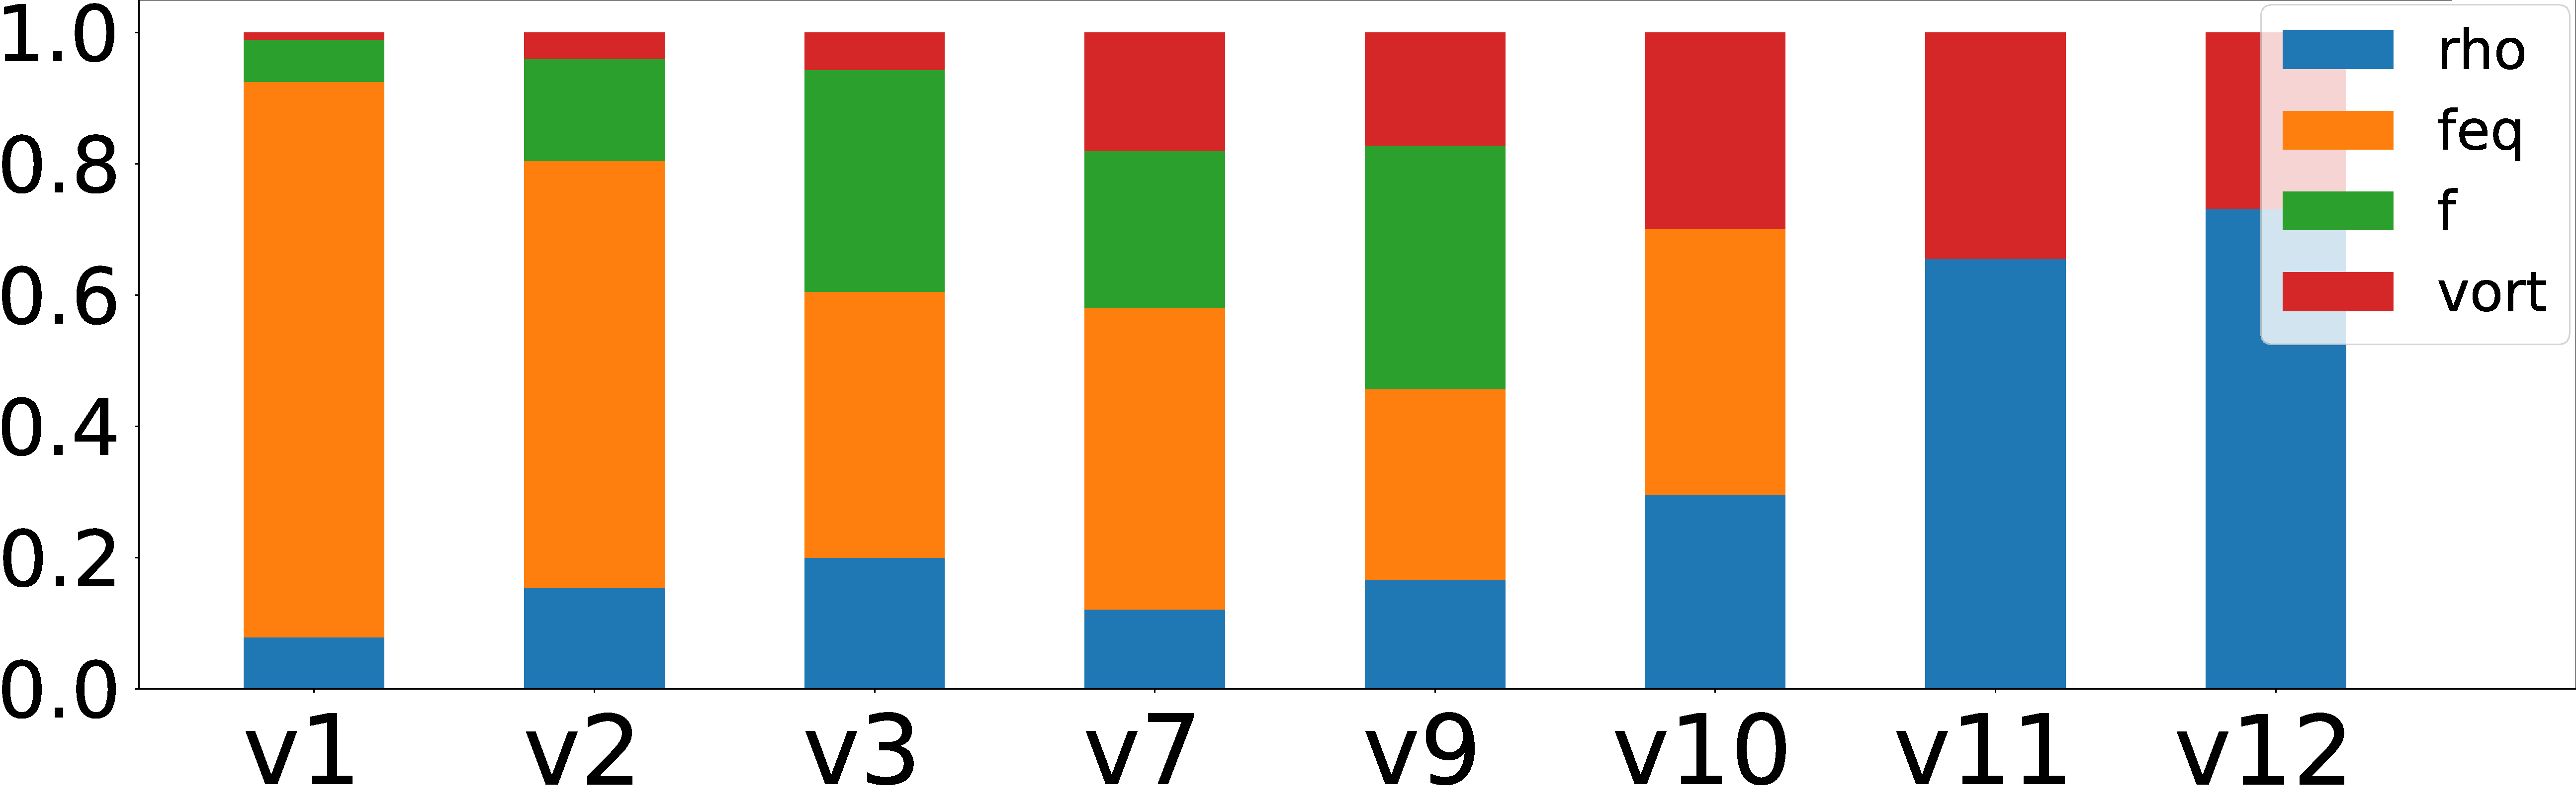
\includegraphics[width=\linewidth]{fig/2D_artifacts/bar_plot_report.out.pdf}
    \caption{Bar plot showing critical paths in the 2D computation}
    \label{fig:2D_bar}
\end{figure}

We list the major 2D versions created and analyze their effect.

\begin{enumerate}[label=\textbf{V\arabic*:}]
    % \setcounter{enumi}{-1}
    \item This is the base implementation after having been translated from Python to C.
    \item
    In this version, we unrolled the boundaries of the loop calculating the vorticity, which eliminated numerous modulo operators in their array indexes.
    This resulted in a much better performance of the vorticity calculation.
    \addtocounter{enumi}{5}
    \item
    Here, some constants were cleaned up, resulting in certain calculations to be precomputed and already resolved by the preprocessor, instead of having to recalculate them during runtime.
    \item Similar to \textbf{V2}, we unroll the drift-loop at its boundaries, allowing us to get rid of modules, resulting in a faster processing speed of the drift step.
    \item
    In this version, we vectorized F and FEQ by hand and subsequently merged the two computations together.
    This caused a significant speedup due to more efficient utilization of SIMD instructions, as well as better temporal locality, due to immediately utilizing the newly calculated values for \texttt{F} for calculating \texttt{FEQ}, instead of having them separated over two loops.
    \item
    Here, we went on to vectorize the calculation of \texttt{Rho} and merged it with the \texttt{F/FEQ} calculation.
    For the same reasons as for \textbf{V10}, this caused a noticeable increase in performance.
    \item
    In this final version, we optimized the collision object to no longer be a boolean matrix indicating which points of the grid are part of it, but rather an array of the indexes themselves.
    
    \item
    This version was branched off of V9 and used shadow indexing instead of rolling the \texttt{F} matrix.  
    While this technique allowed us to save on memory accesses, it disallows vectorization due to the matrix now no longer being 32-byte aligned. Because of this, a drop in performance was observed.
\end{enumerate}

The final version has minimal memory accesses, only using them for rolling the matrix \texttt{F} and later fetching the values of \texttt{F} and storing the results back in \texttt{F} and \texttt{Vort}.  
Further computations cannot be eliminated without breaking the algorithm, and their computation cannot be further sped up due to them already being vectorized and common sub-expressions being reused.  

The final performance falls below the theoretical bound when accounting for the instruction mix, which is around 9.15 flops/cycle.
Our final performance of around 6 flops/cycle can be explained by stalls coming from dependencies within the calculation.

\mypar{3D Implementation} The chosen 3D baseline is implemented in C++. We therefore first translated it to pure C. The initial work consisted again of cleanup and trivial performance improvements, such as removing redundant libraries, option parsing and freeing memory between runs. This is what we named v0. We used the periodic boundary condition, as this is what was used in 2D too.

Similar to the 2D version, we generate a bar plot for identifying the computation's bottlenecks, helping us more efficiently focus our efforts on the parts most responsible for lowering performance.

\begin{figure}[h!]
    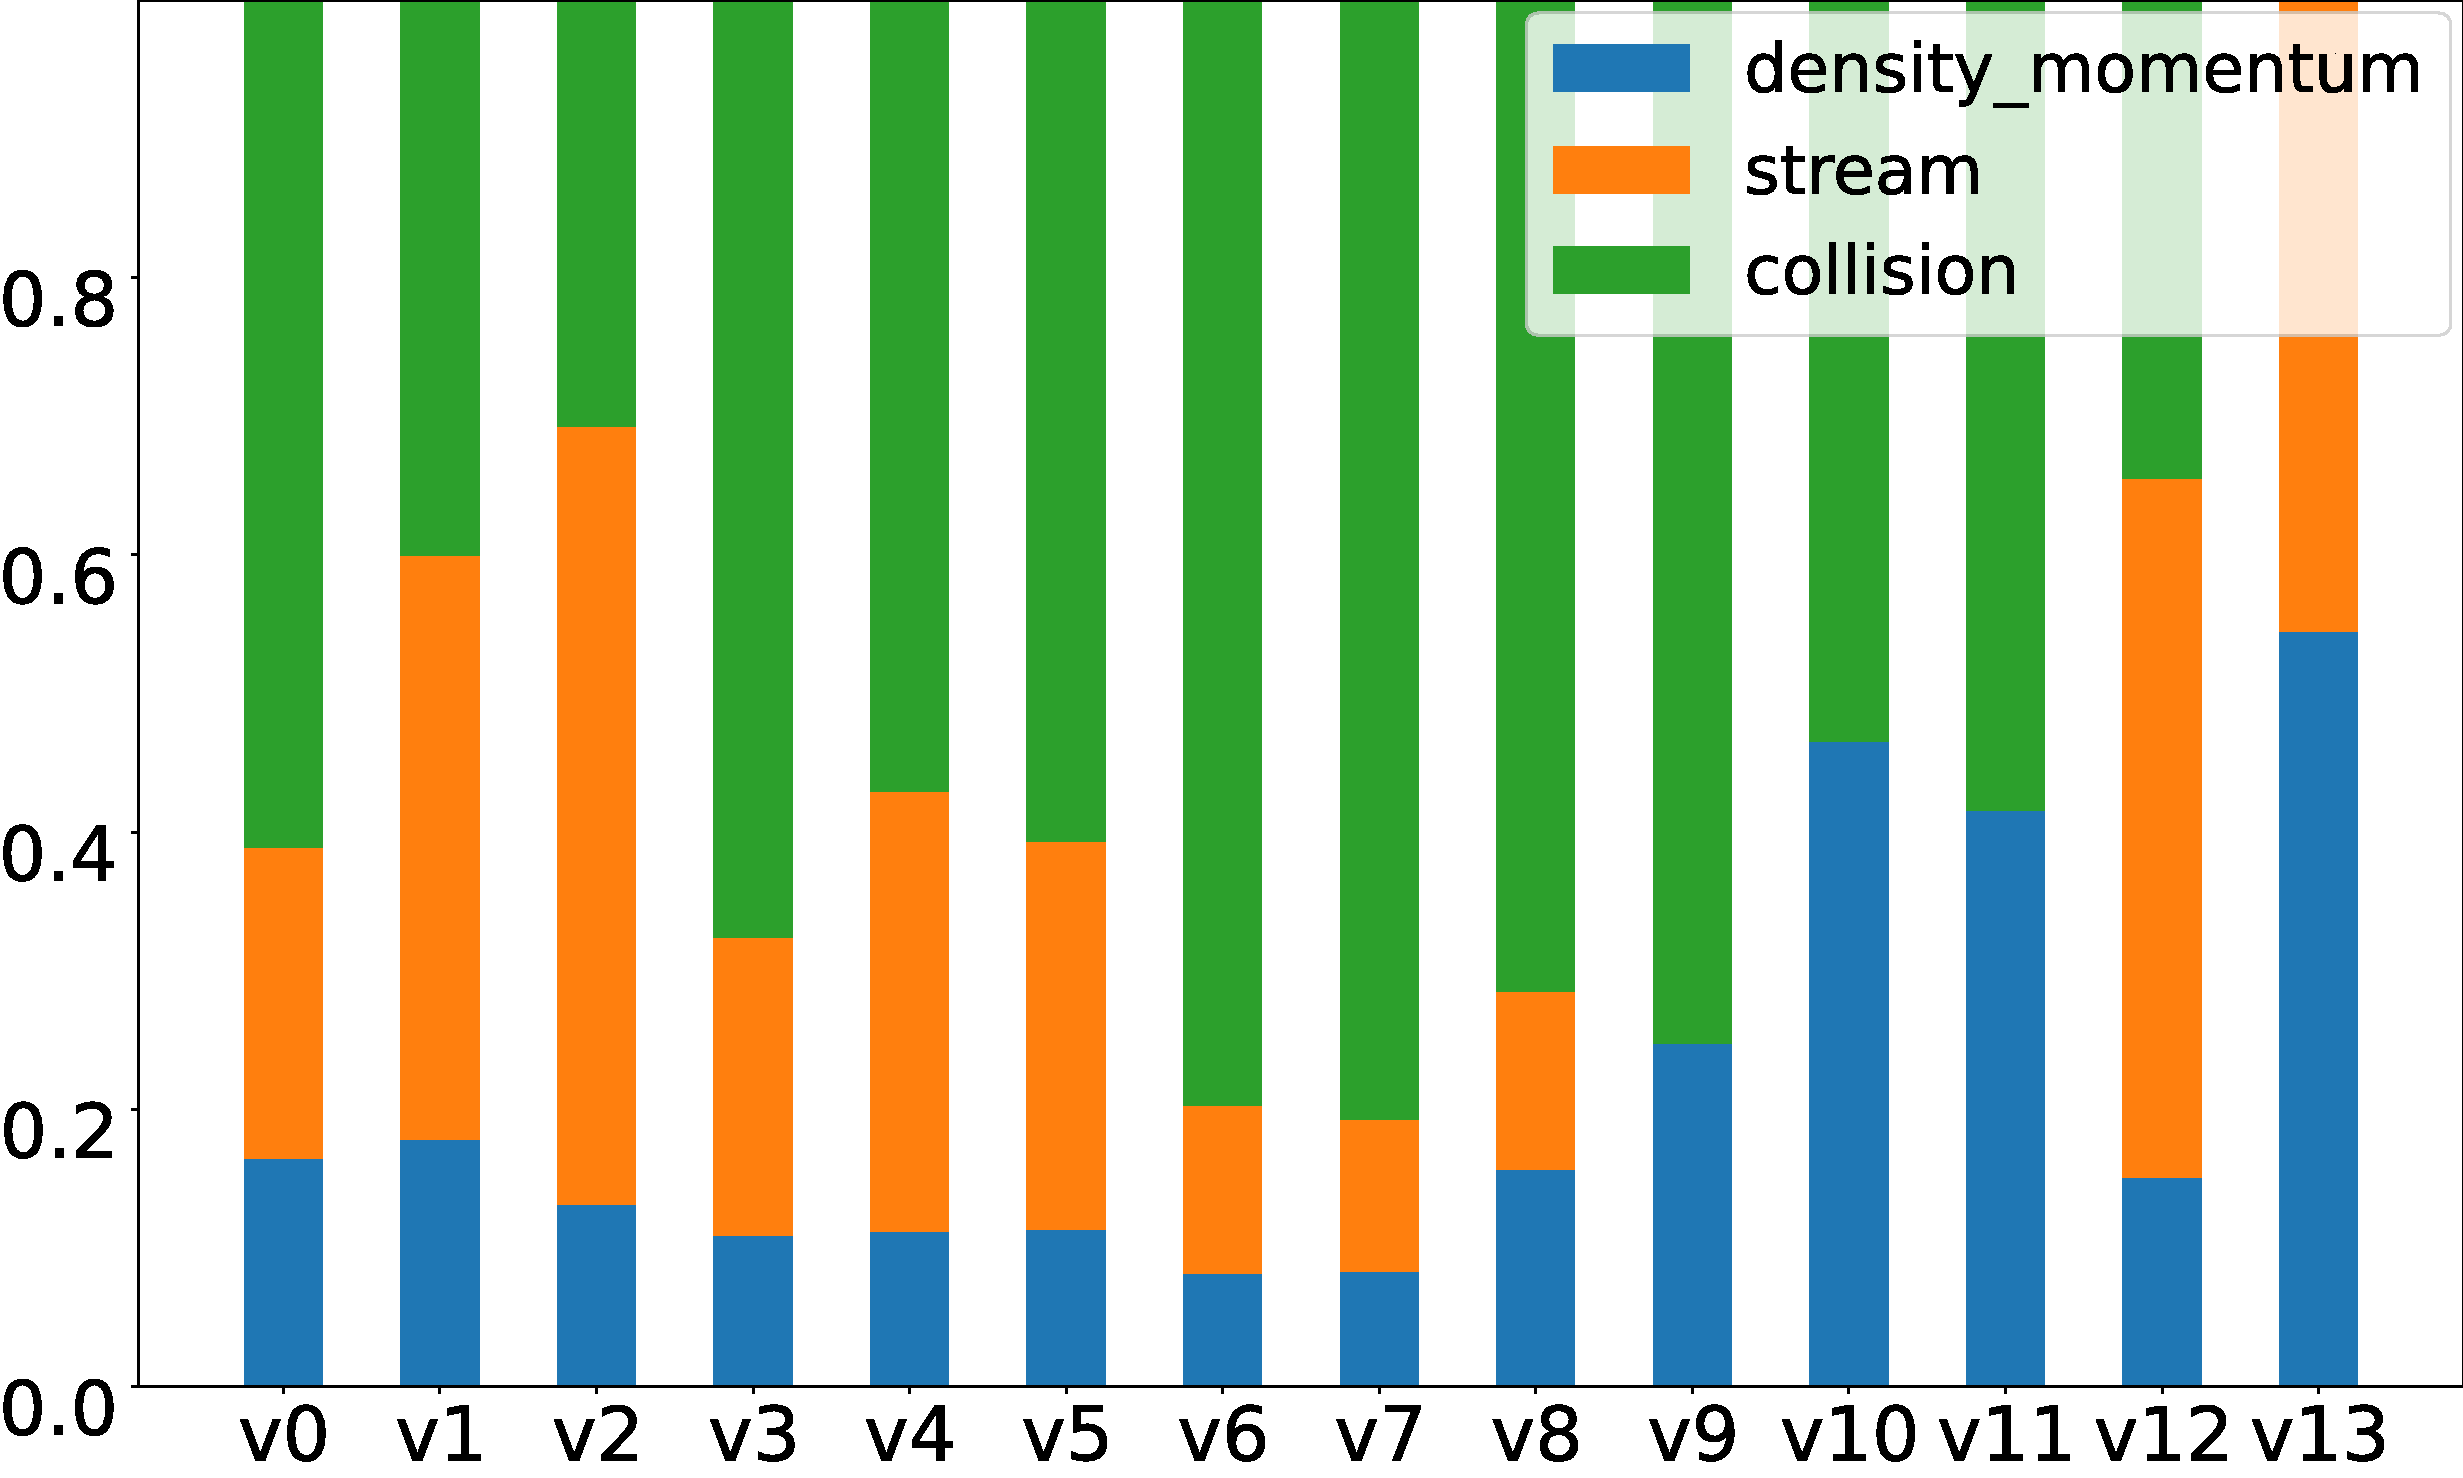
\includegraphics[width=\linewidth]{fig/3D_artifacts/bar_plot_report.out.pdf}
    \caption{Bar plot showing critical paths in the 3D computation}
\end{figure}
\begin{enumerate}[label=\textbf{V\arabic*:}]
    \setcounter{enumi}{-1}
    \item This is the base implementation.
    \item We started defining the parameters at compile time so that we could test and benchmark with various inputs. 
    \item Here we noticed that our computation was highly memory-bound. This can be easily explained by the order of the for-loops, as we were accessing the data in a chaotic order. After this, all accesses were consecutive in memory. This step also illustrated that we won't benefit from blocking in the loops, as the data was already accessed in a favourable manner.
    \item We started simplifying the operations in \texttt{FEQ} - removing repeated expressions, exchanging divisions for multiplications, and similar. As the \texttt{FEQ} operation happens in the collision step, we can see that its proportion gets smaller in the bar plot.
    \addtocounter{enumi}{1}
    \item Here we removed all the constant arrays, which also included some loop unrolling. As this leads to some multiplications with zero or one, we also could reduce the number of flops.
    \item We made sure that all of the loop unrolling for above has a sufficient number of accumulators and unrolled further.
    \item We noticed that the stream was taking a large number of cycles, although it consists only of data movement. Thus we changed the order of modulo operations around so that the memory accesses are in a more favourable order but this caused overcomplication of the code and no improvement.
    \addtocounter{enumi}{1}
    \item We implemented dynamic indexing, where instead of moving data in the stream, we calculate the index used based on the current step. This caused an improvement, as we removed the whole stream function but it rendered the code un-vectorizable, as the data for the calculations is misaligned. We tried to further improve it with \textbf{V10} and  \textbf{V11} but we didn't achieve significant improvements.
    \addtocounter{enumi}{1}
    \item We vectorized the code as an alternative to V9 and noticed that it was a lot more beneficial, so we proceeded with it. As it is compute-bound, we tried to improve the memory movements.
    \addtocounter{enumi}{1}
    \item We merged the density compute function and the collision function, which lead to better memory movement.
\end{enumerate}
Further improvements would again include memory movement improvements, but we couldn't find an optimal way to execute them which lead to a significant improvement of the performance. This included merging the two leftover functions into one.

\section{Experimental Results}\label{sec:exp}

\mypar{Experimental setup} 

We rented a dedicated machine to perform our measurements and evaluation. The machine features an AMD Ryzen 7 PRO running at 4.7GHz. The CPU has an L1d and L1i cache size of 256KB each, L2 size of 4MB and L3 of 16MB. 
This CPU supports AVX-256 instructions.
We set it up as a Gitlab Pipeline runner such that for each commit the machine would test for consistent results with the baseline and the absence of memory leaks, benchmark each version and generate all the plots. Convenient Makefiles were set up for a speedy development cycle. The codebases were compiled using the GCC Compiler v11.4.0 on Ubuntu 22.04.4 LTS. For testing, we compared the current code with the baseline implementation and checked it with a tolerance of $10^{-4}$ from the standard deviation.

To compute the performance and Operational intensity accurately we used PAPI~\cite{mucci1999papi} which leverages hardware counters to retrieve the exact count of flops and memory movements. It also supports sectioning the code, allowing us to measure parts of the implementation separately from one another to identify bottlenecks. One of its downsides is that it can only estimate memory movements from disk to RAM, but not in the cache itself for our model processor.\\

For measuring cycles taken, we also wrote our profiler. It runs parts of the code multiple times and takes the average number of cycles for it. In this case, we partitioned the code into different functions which we evaluated separately.

When benchmarking, we compile a version of the executable with PAPI enabled and one without.
Due to PAPI causing an overhead during execution, including it in the executable profiling the used cycles would negatively impact results.

For benchmarking, we used a wide range of input sizes varying and varied the spatial dimensions. The parameters differed between 2D and 3D, but the primary constraints were that input sizes needed to be divisible by 4. This allows vectorization and saturation of the application's full L3 cache, allowing us to observe the performance impacts of cache misses, with additional sizes mostly residing in the main memory.


We used various flags while working on the code and observed that, for the 3D version, most flags enabling fast math resulted in higher tolerance deviations. This was due to the numerous floating-point operations in our code, whose order would change with these flags. Ultimately, for 2D we enabled the \texttt{-Ofast} \texttt{-floop-nest-optimize} \\\texttt{-ffinite-math-only} flags and for 3D \texttt{-Ofast}  \\\texttt{-march=native}  \texttt{-mavx}  \texttt{-mfma}, also maintaining a tolerance of $10^{-4}$ from the baseline.


\mypar{Results}
\begin{figure}[h!]
\begin{subfigure}[t]{\linewidth}
    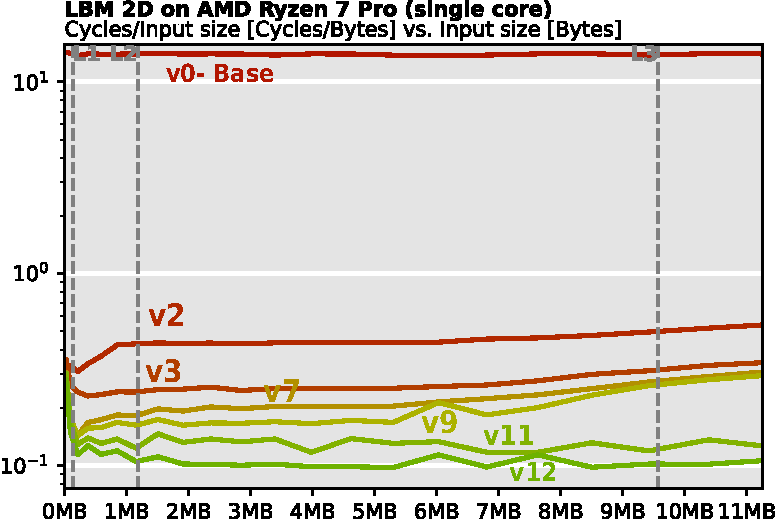
\includegraphics[width=\linewidth]{fig/2D_artifacts/sizevscycles_report.out.pdf}
    \caption{2D version}
\end{subfigure}
\begin{subfigure}[t]{\linewidth}
    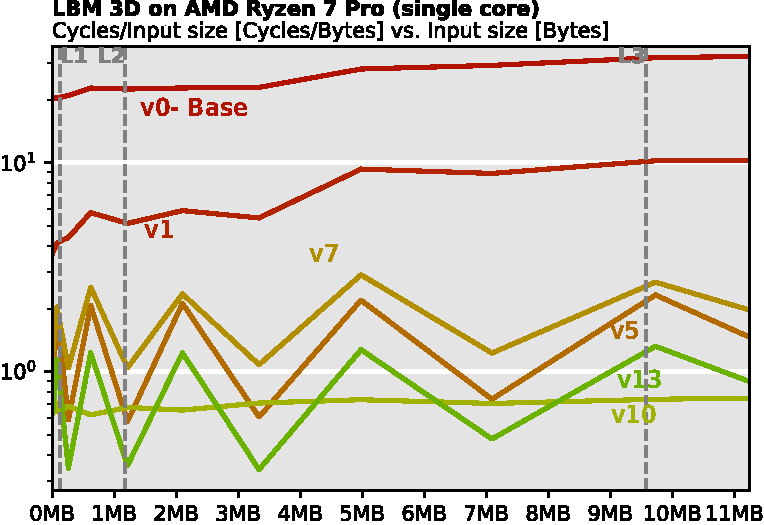
\includegraphics[width=\linewidth]{fig/3D_artifacts/sizevscycles_report.out.pdf}
    \caption{3D version}
\end{subfigure}
    \caption{Runtime to input size ratio plots. Lines higher up on the y-axis take more cycles for each input byte, thus having worse performance.}
\label{fig:sizevcycle}
\end{figure}


In Figure~\ref{fig:sizevcycle}, we show how the optimizations we applied affected the cycle count per byte of input. Since the amount of flops and memory transfer changed between versions, this was very useful for putting our work into perspective in terms of efficiency achieved. We increment the inputs by multiplying X, Y and Z with constants.

For 2D, we see the gradual improvement of the optimizations we apply.
Especially when looking at larger input sizes, a clear jump in performance can be seen in the second-latest version, which is where manual vectorization was applied. 

For the 3D version, we have a very interesting behaviour, as the set of data we use at one time stops fitting into the cache. We happen to fit into it just fine with some input sizes but not for others which depends on the exact values of X, Y and Z (which we multiply with constants). This is also why V11 doesn't show this behaviour - it is already memory-bound by the collision step.

\begin{figure}[h!]
\begin{subfigure}[t]{\linewidth}
    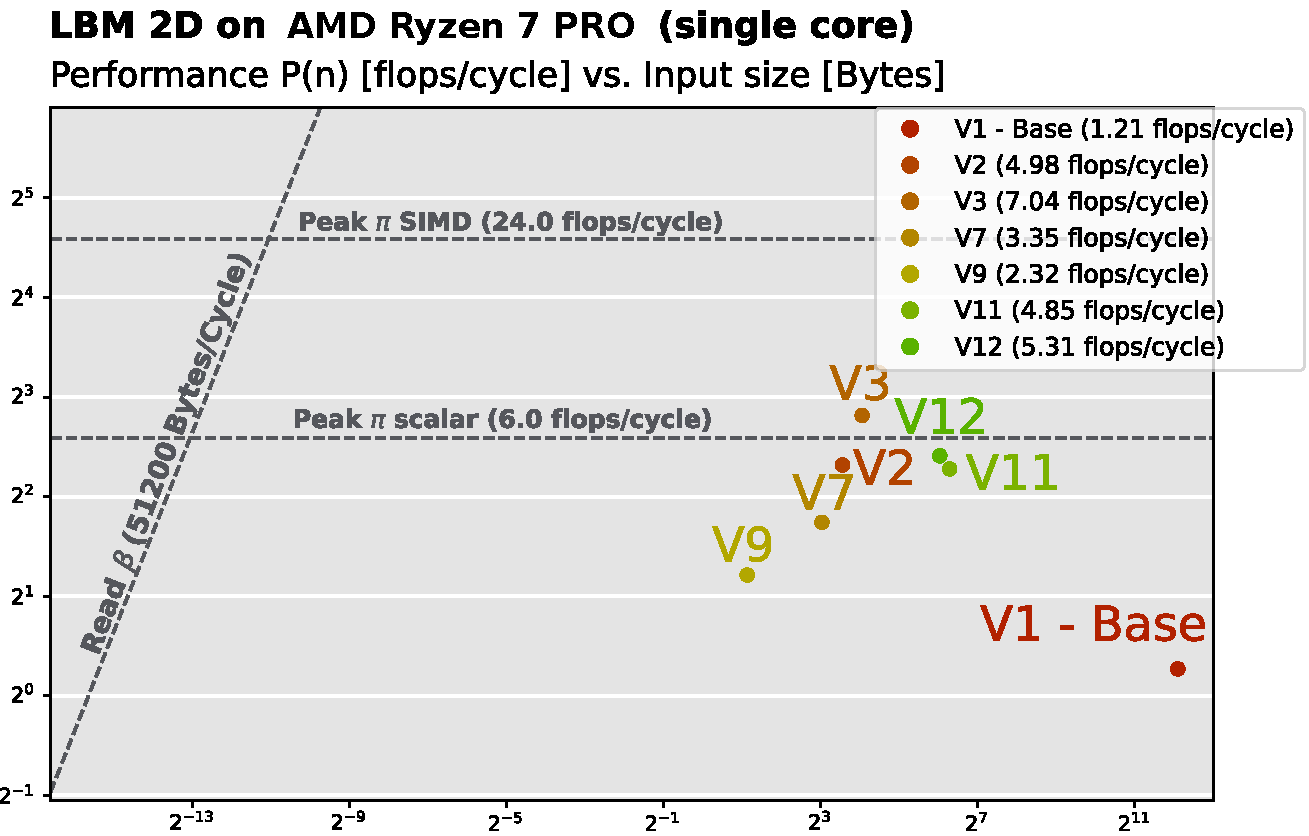
\includegraphics[width=\linewidth]{fig/2D_artifacts/roofline_plot_report.out.pdf}
    \caption{2D version}
\end{subfigure}
\begin{subfigure}[t]{\linewidth}
    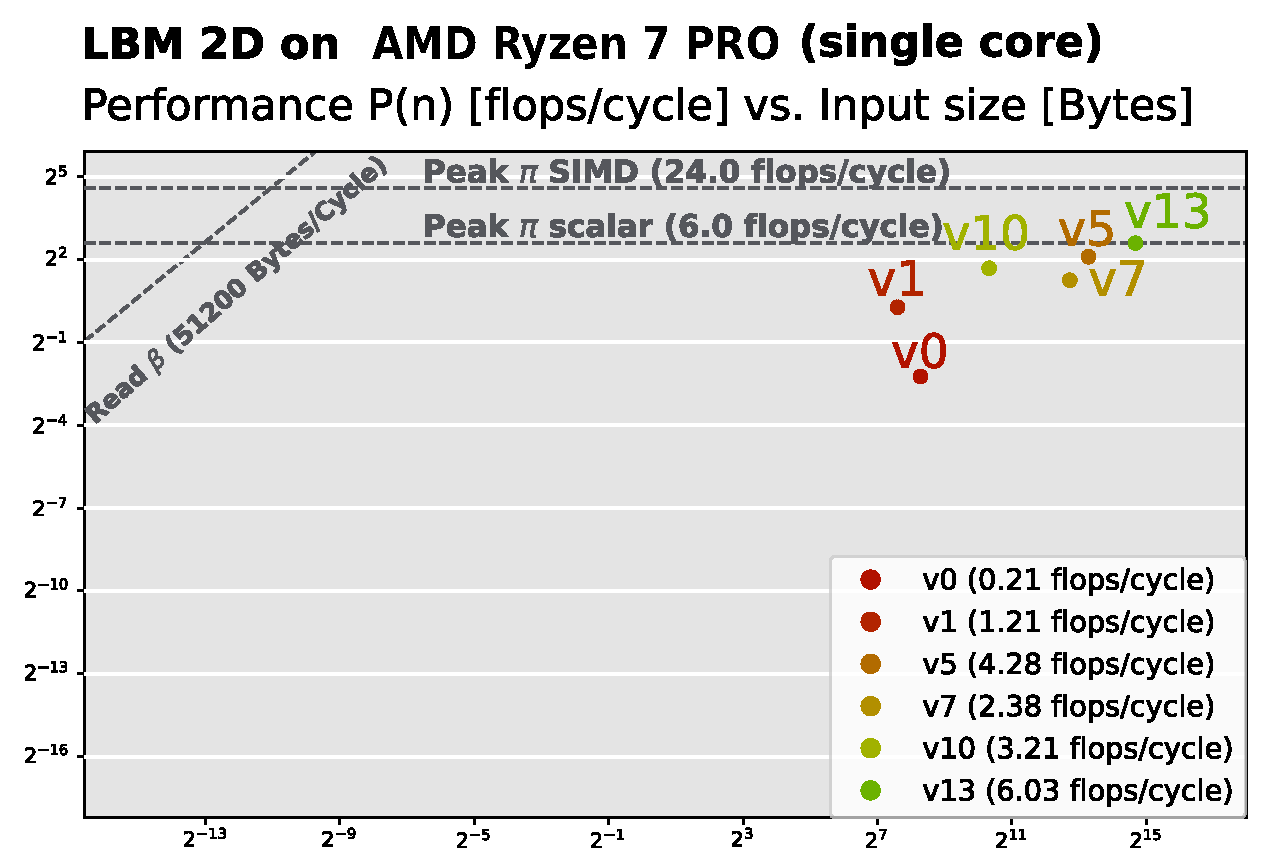
\includegraphics[width=\linewidth]{fig/3D_artifacts/roofline_plot_report.out.pdf}
    \caption{3D version}
\end{subfigure}
    \caption{Roofline plots, with the read being the bandwidth of reading from disk to RAM}
    \label{fig:rooflines}
\end{figure}

Figure~\ref{fig:rooflines} shows the roofline plots we created of our different versions.
They were again useful for estimating the effectiveness of our algorithm and show its gradual improvement.
Another important metric in them is the flops per cycle in the legend.
For their creation, we used data gathered from PAPI, which showed the exact number of flops and bytes transferred from the main memory.
However, PAPI could only track the amount of data moved from RAM to the CPU, with there not being any way of accurately tracking movements within the caches themselves for Zen3, even with other tools.

For both 2D and 3D, we notice that most of the versions have a high arithmetic performance, lying far away from being memory-bound.
The plot also shows where we managed to get rid of flops, such is the case when comparing 2D's \textbf{V3} to \textbf{V7}.  
Due to \textbf{V7} having fewer flops, its performance seems to decrease despite the actual computation being shorter when compared to \textbf{V3}.

\section{Conclusions}

In this paper, we have optimized the Lattice Boltzmann Method (LBM) for AMD Zen3 CPUs.
We have shown how we proceeded with the optimizations for both the 2D and 3D versions of LBM, where both versions led to unique issues surfacing.  
Ultimately, we managed to achieve around a 2.5x speedup for both the 2D and 3D implementation over the baseline when both versions are compiled using optimal compiler flags.

\section{Further comments}
\mypar{3D baseline issues} We realized after a while that the 3D baseline was deeply flawed, in which it performed the stages in each timestep in the wrong order. By doing so, the baseline was overriding the initial conditions resulting in a homogeneous vorticity output rendering the simulation useless. Furthermore, the MATLAB visualization script was returning an exception upon compiling because of wrong addressing in the code. We therefore fixed the 3D baseline by applying modifications to both the simulation script and the visualization script.

\mypar{3D unexpected flags behaviour}
When testing out compiler flags for the 3D version, we noticed that combining \texttt{-march=native} and \texttt{-Ofast} resulted in extreme numerical instability, leading to a chaotic result.
Due to this, some versions had to use only the \texttt{-Ofast} flag, and required the use of \texttt{-fno-fast-math}, in order to ensure numerical stability.

\mypar{Boundary condition} At the beginning we also tried out the couette boundary condition but re-indexing it for removing stream proved to be very troublesome, so we decided to go with periodic.


\section{Contributions of Team Members (Mandatory)}

% \INFO{
% In this mandatory section (which is not included in the 7 pages
% limit) each team member should very briefly (telegram style is
% welcome) explain what she/he did for the project. I imagine
% this section to be maximally one column. Do not put any
% appendix besides that.
% Include only
% • What relates to optimizing your chosen algorithm / application. This means writing actual code for optimization or for analysis.
% • What you did before the submission of the presentation.
% Do not include
% • Work on infrastructure and testing.
% • Work done after the presentation took place.
% Example and structure follows.
% Marilyn. Focused on non-SIMD optimization for the
% variant 2 of the algorithm. Cache optimization, basic block
% optimizations, small generator for the innermost kernel (Section 3.2). Roofline plot. Worked with Francois on the SIMD
% optimization of variant 1, in particular implemented the bitmasking trick discussed.}

% \mypar{Dominic} Infrastructure
% Researched and implemented accurate flop counting and
% memory transfers
% Researched hardware and calculated max perf based on
% instruction mix
% Implemented the cycles profiler
% Implemented the candle-bar plotting
% Further improved plotting through better automation
% 2D
% All of the Vectorization
% Shadow indexing
% Unrolling boundary conditions in vorticity and drift
% Improved storing of collision cells
% 3D
% All of the Vectorization


% \mypar{Kamelia} Infrastructure
% initial 3D version + initial benchmark/plot
% 2D refactorization of the code (to make it similar to 3D)
% Try different flags
% 2D
% Remove constant arrays
% Loop unrolling
% Optimize mathematical computations
% 3D
% Change order of for-loops, unroll, remove dependencies
% Optimize mathematical computations
% Remove constant arrays, change data structures
% Start up shadow indexing and try it out with couette boundary condition


% \mypar{Albert} 
% 2D/3D Makefile/CMake for plotting, compiling every version, testing against baseline, checking for memory leaks
% 2D/3D Benchmark plot script
% 2D/3D Size vs Cycles plot script
% 2D/3D Compare script
% Established 2D pipeline and pipeline runner for automatic validation/plotting

% Initial 2D initialization optimizations
% 3D Streaming improvements
% Compile-time defined parameter optimization
% Memory access pattern optimization on F


% \mypar{Karlo}
% Won the lucky 25\% win to present :>
% Initial 2D python -> C/C++ translation
% Initial Compare script
% 2D/3D Plotting/Benchmarks
% Visualization
% 3D Streaming improvements
% 3D Shadow indexing to remove unnecessary data movements

\mypar{Dominic}
Focused on optimizing 2D and 3D algorithms. Implemented vectorization for both dimensions. Applied shadow indexing for 2D, unrolled boundary conditions in vorticity and drift, and improved collision cell storage. Developed cycles profiler and enhanced plotting automation with candle-bar plots. Researched accurate profiling and added PAPI.

\mypar{Kamelia}
Initialize 3D version. Optimized both 2D and 3D code. Refactored 2D to align with 3D structure, removed constant arrays, and unrolled loops. Improved mathematical computations and data structures. Applied shadow indexing with periodic boundary condition for 3D.

\mypar{Albert}
Optimized 2D initialization and 3D streaming. Refined memory access patterns on F and compile-time parameter optimization. Created scripts for benchmarking, plotting, and comparison across 2D and 3D versions.

\mypar{Karlo}
Translated initial 2D code from Python to C/C++. Improved 3D streaming and implemented shadow indexing to eliminate unnecessary data movements. Contributed to plotting and benchmarking for both 2D and 3D.


% References should be produced using the bibtex program from suitable
% BiBTeX files (here: bibl_conf). The IEEEbib.bst bibliography
% style file from IEEE produces unsorted bibliography list.
% -------------------------------------------------------------------------
\newpage

\balance
\bibliographystyle{IEEEbib}
\bibliography{bibl_conf}

\end{document}